\section{Introduction}

SciVis is interdisciplinary the fields of application include engineering, natural sciences and medical sciences.   There's a common application to all fields: 
There are \emph{numerical datasets} providing an abstraction from the particular application. The characteristics of such datasets include:
\begin{description}
\item[Dimension of domain:] Number of coordinates or parameters
\item[Dimension of values:] Scalar, vector or tensor fields
\item[Type of data:] Discrete values versus discretised data
\item[Type of discretisation:] (Un-)structured grid, scattered data
\item[Time dependencies:] Static versus time-dependent.
\end{description}

\subsubsection{SciVis and InfoVis}
\begin{description}
    \item[Scientific Visualisation] is mostly concerned with 
        \begin{itemize}
            \item 2,3,4 dimension spatial or spatio-temporal data
            \item discretised data
        \end{itemize}
    \item[Information Visualisation] focuses on:
        \begin{itemize}
            \item High-dimensional, abstract data
            \item Discrete data
            \item Financial, statistical, etc.
            \item Visualisation of large trees, networks, graphs
            \item Data mining:
                \begin{itemize}
                    \item Finding patterns
                    \item Clusters
                    \item Voids
                    \item Outliers
                \end{itemize}
                
        \end{itemize}

\end{description}

\subsection{Visualisation Scenarios}
The reference model for visualisation:
\begin{figure}[H]
    \centering
    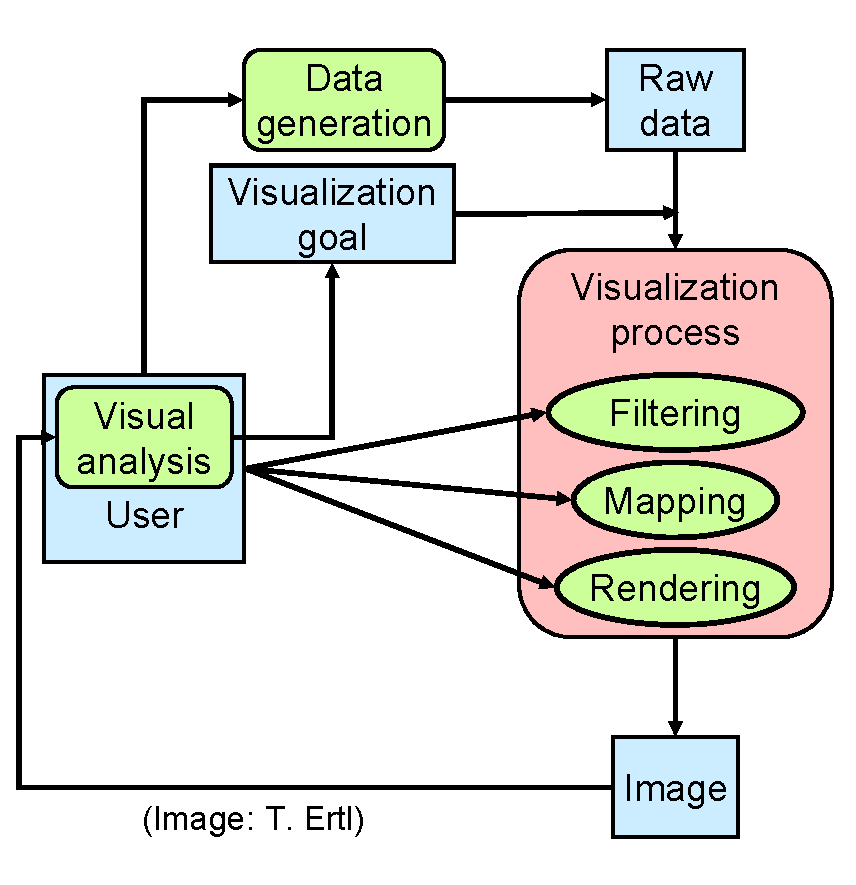
\includegraphics[width=0.5\textwidth]{img/01_vis_scenarios}
\end{figure}
\subsubsection{Video/Movie}
In a first step the data is generated. Then the data is visualised during a batch visualisation step and in the end the video is analized. 
\begin{figure}[H]
    \centering
    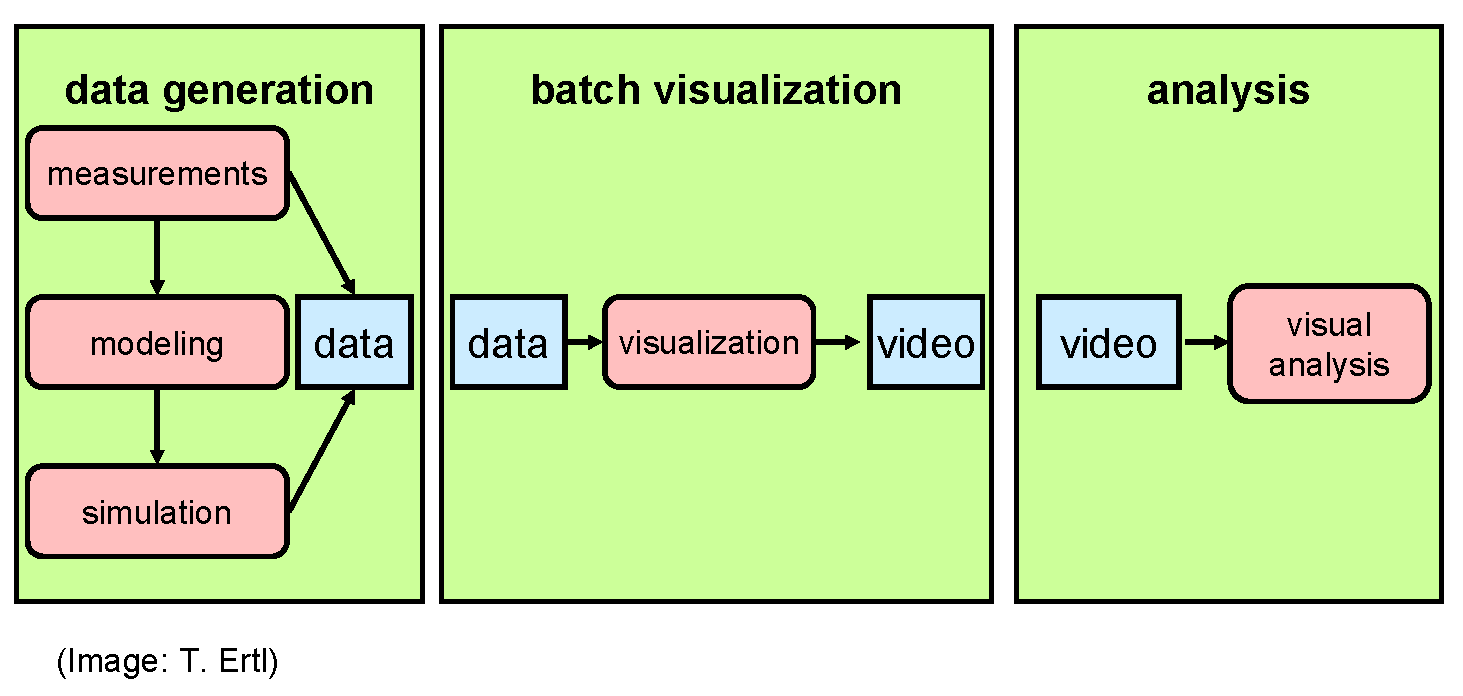
\includegraphics[width=0.75\textwidth]{img/01_movie_mode}
\end{figure}

\subsubsection{Tracking}
The gathered data is directly visualised and analysed.
\begin{figure}[H]
    \centering
    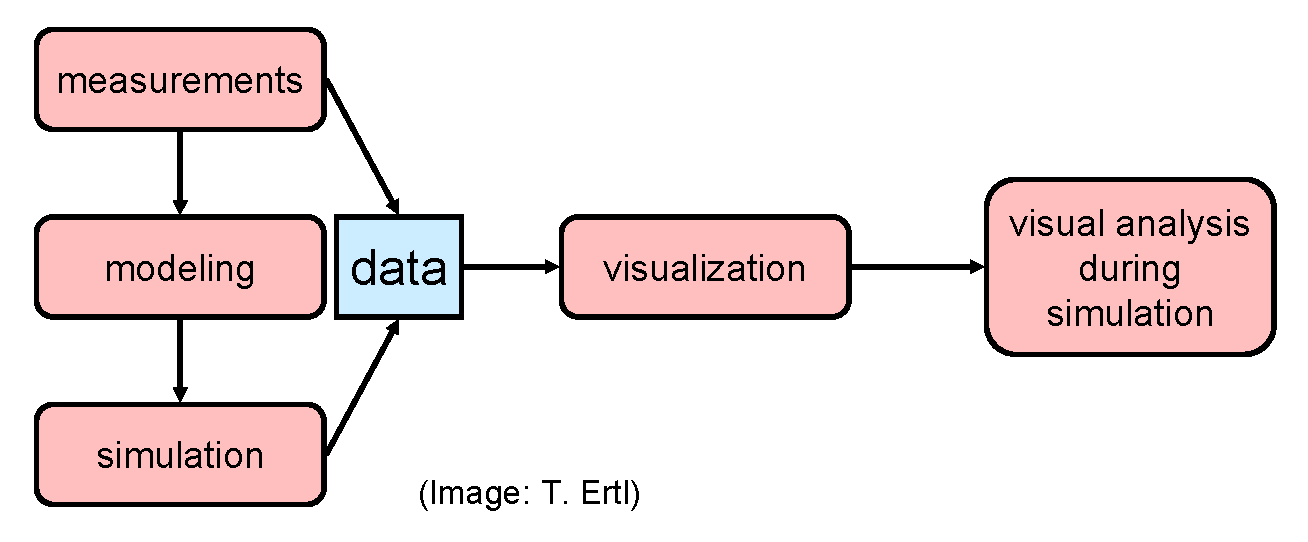
\includegraphics[width=0.75\textwidth]{img/01_tracking}
\end{figure}
\subsubsection{Interactive Post Processing/Visualisation}
The data generation step is split from the visualisation step. 
\begin{figure}[H]
    \centering
    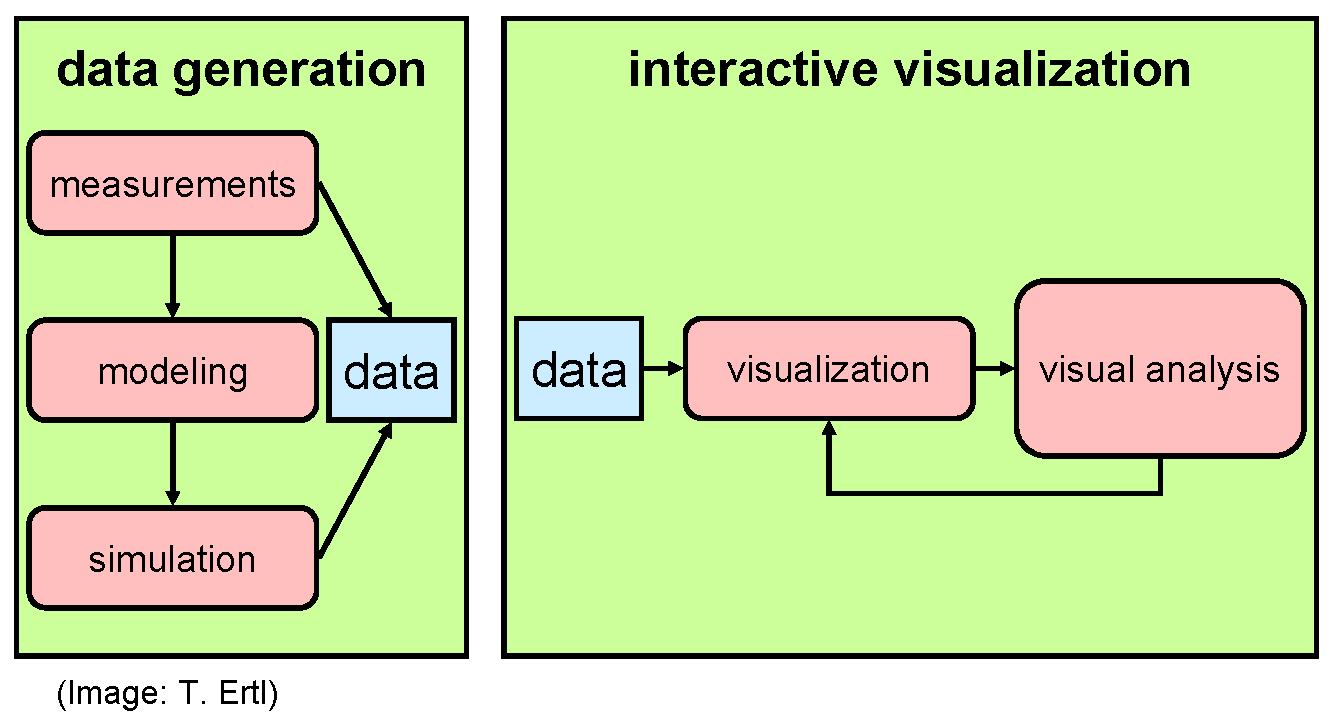
\includegraphics[width=0.75\textwidth]{img/01_interactive_post}
\end{figure}
\subsubsection{Interactive Steering/Computational Steering}
The visualisation has a direct impact on the simulation and the visualisation.
\begin{figure}[H]
    \centering
    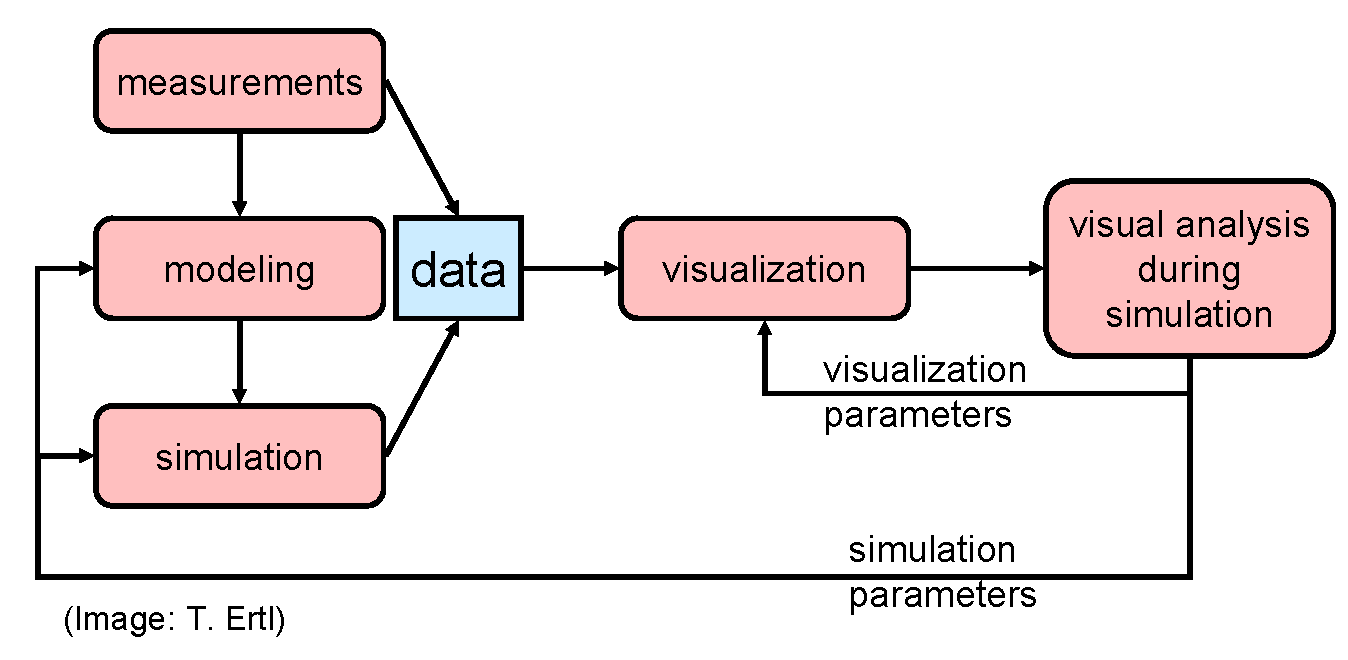
\includegraphics[width=0.75\textwidth]{img/01_interactive_steering}
\end{figure}

\subsection{Data Discretisations}
Types of data sources have typical types of discretisations:
\begin{description}
\item[Measurment Data] Typically scattered ("mesh-less", no grid)
\item[Numerical Simulation Data] $\ $
    \begin{itemize}
        \item Structured, block-structured or unstructured grids
        \item Adaptively refined meshes
        \item Multi-Zone grids with relative motion
        \item ...
    \end{itemize}
\item[Imaging Methods] Uniform grids
\item[Mathematical Functions] (and functionally represented data) can be sampled by demand:
    \begin{itemize}
        \item Uniform
        \item Adaptive
    \end{itemize}
\end{description}

\subsection{Unstructured Grids}
\subsubsection{2D Unstructured Grids}
Cells are \emph{triangles} and/por quadrangles. The domain can be a surface embedded in $3$-space (distinguish $n$-dimensional from $n$-space).
\begin{figure}[H]
\centering   
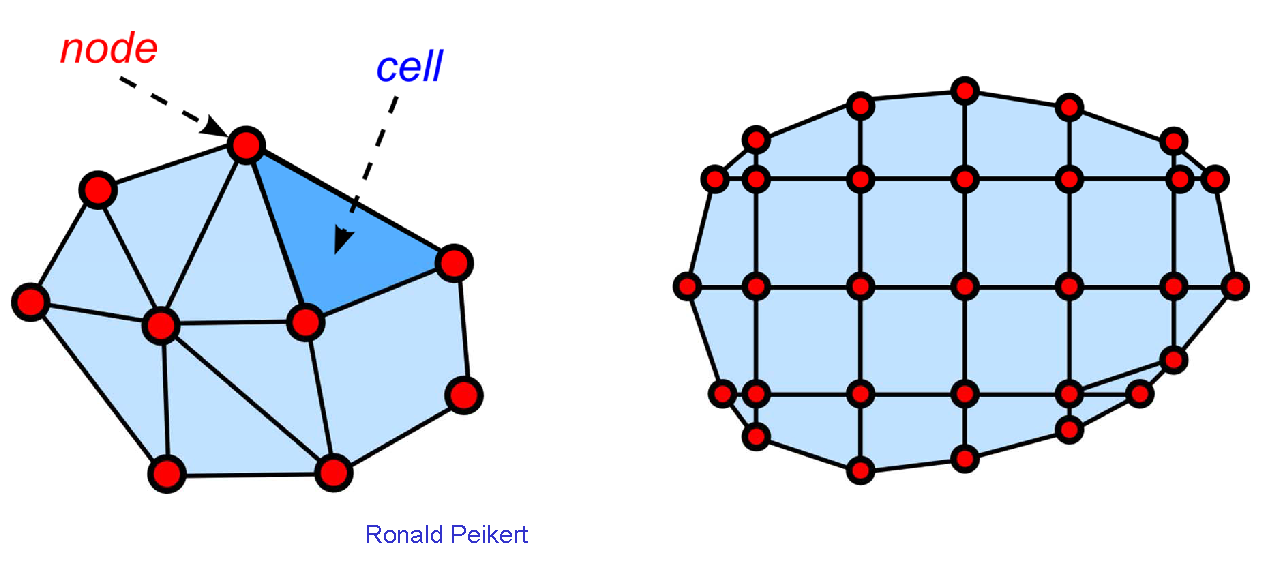
\includegraphics[width=0.75\textwidth]{img/01_unstructured_grids}
\end{figure}

\subsubsection{3D Unstructured Grids}
Cells are \emph{tetrahedra} or \emph{hexahedra}.
\begin{figure}[H]
\centering
\includegraphics[width=0.6\textwidth,page=2]{img/01_3d_unstructured_grids}
\end{figure}
Mixed grids ("zoo meshes") require additional types:
\emph{wedge} ($3$ sided prism), and a \emph{pyramid} ($4$-sided).
\begin{figure}[H]
\centering
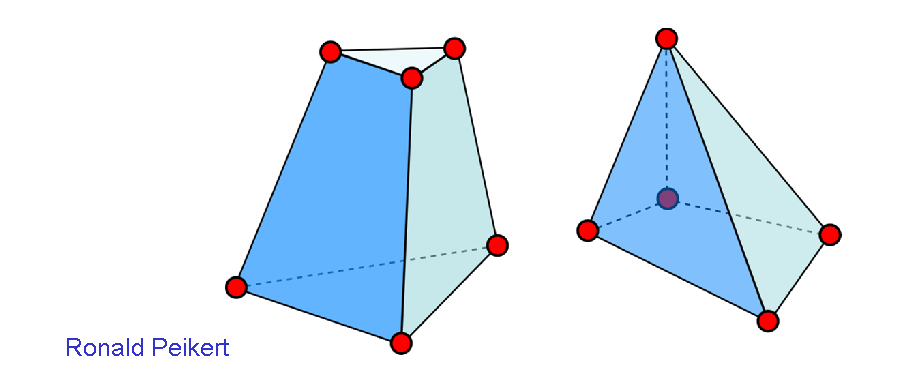
\includegraphics[width=0.6\textwidth,page=1]{img/01_3d_unstructured_grids}
\end{figure}

\subsection{Structured Grids}
\begin{description}
    \item[Curvilinear Grid (general case)] Nodes are given in an array $N_i\times N_j\times N_k$ and the cells are implicit.
    \begin{figure}[H]
        \centering
        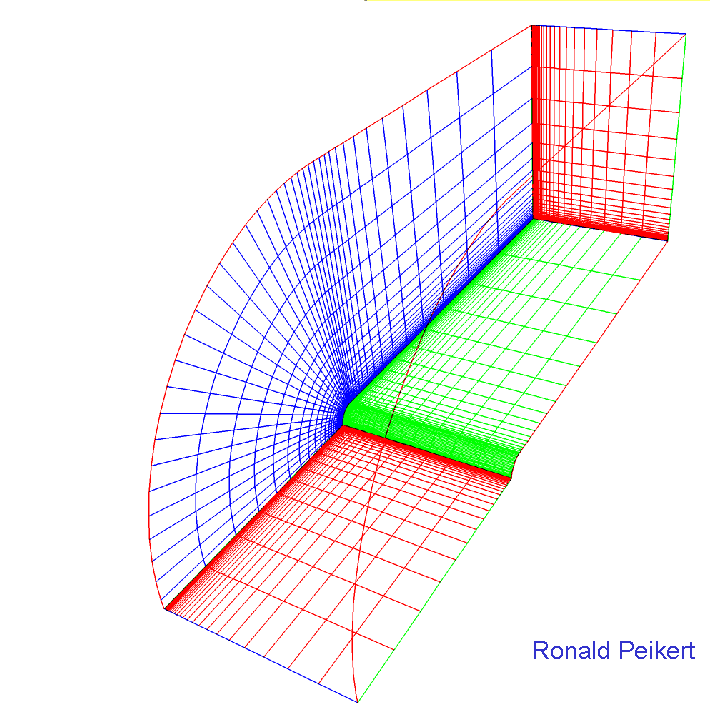
\includegraphics[width=0.5\textwidth]{img/01_curvilinear_grid}
        \caption{Curvilinear Grid}
    \end{figure}

    \item[Rectilinear Grid (special case)] The coordinate functions are simpler:
        \begin{align*}
            x = x(i)\qquad
            y = y(j)\qquad
            z = z(k)
        \end{align*}
        \begin{figure}[H]
            \centering
            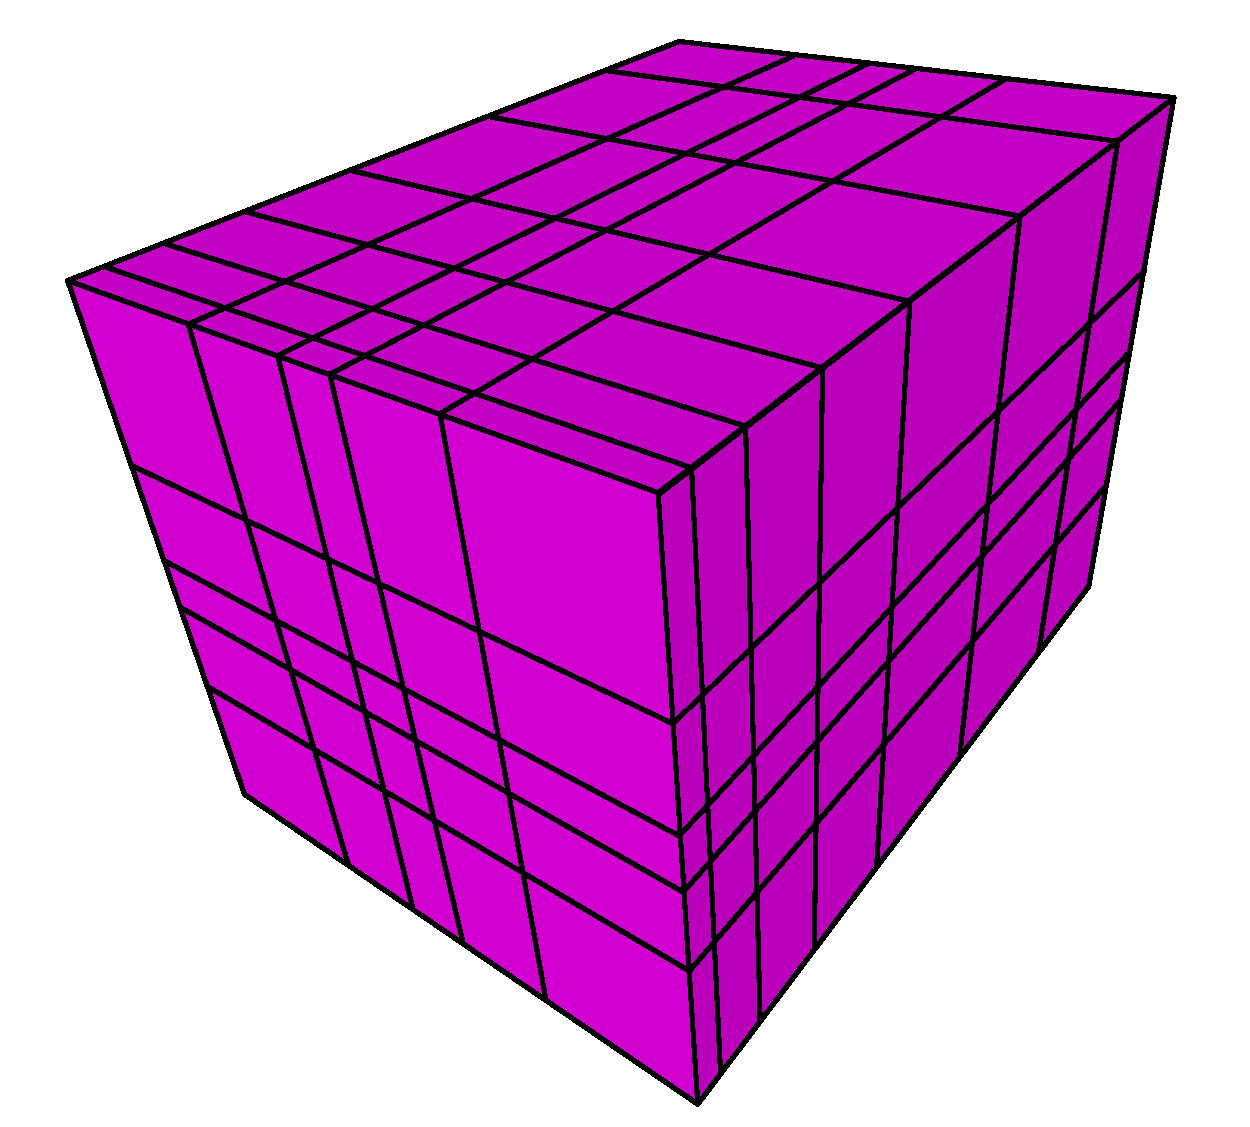
\includegraphics[width=0.25\textwidth]{img/01_rectilinear_grid_wikipedia}
            \caption{Rectilinear Grid, Source: Wikipedia}
        \end{figure}

     \item[Uniform Grid (more special)] The coordinates are defined by an \emph{axis-aligned} bounding box.
\end{description}

\subsubsection{Point-Sampled Data/Scattered Data}
Point sampled data  returns only nodes and no cells. Typical data sources are measurement data for example meteorological data.

Options for visualisation include:
\begin{description}
\item[Point-Based Methods] (relatively few algorithms)
\item[Triangulation] for example constrained Delaunay (difficult in 3D)
\item[Resampling] onto uniform grid.
\end{description}

\subsection{Elementary Visualisation Methods}
\emph{Scalar Fields} can be visualised by plotting its \emph{function graphs}:
\begin{description}
    \item[1D Field:] The Graph is a curve:
        \begin{align*}
            y = f(x)
        \end{align*}
    \item[2D Field:] The Graph is a \emph{height field}:
        \begin{align*}
            z = f(x,y)
        \end{align*}
        Visualisation is easy for rectilinear grids:\\
        \emph{Painter's algorithm} (hidden surface removal in software): Draw cells row by row from back to front.
        \begin{figure}[H]
            \centering
            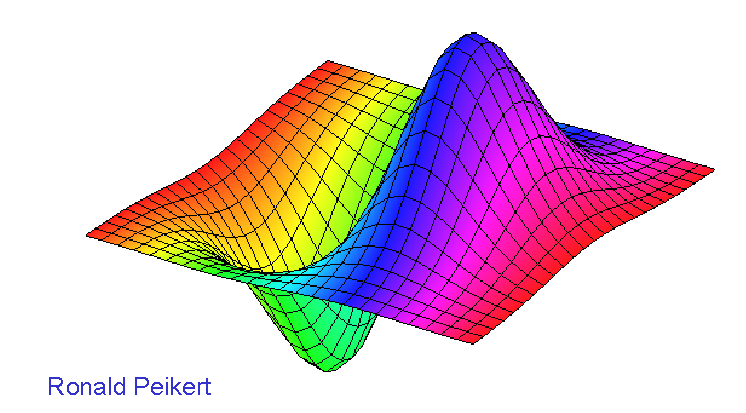
\includegraphics[width=0.7\textwidth]{img/01_painters_algorithm}
        \end{figure}
\end{description}

Scalar fields can also be visualised using \emph{color coding} using \emph{1D texture mapping}. Don't use \emph{vertex colors} and Gouraud shading!
\begin{figure}[H]
    \centering
    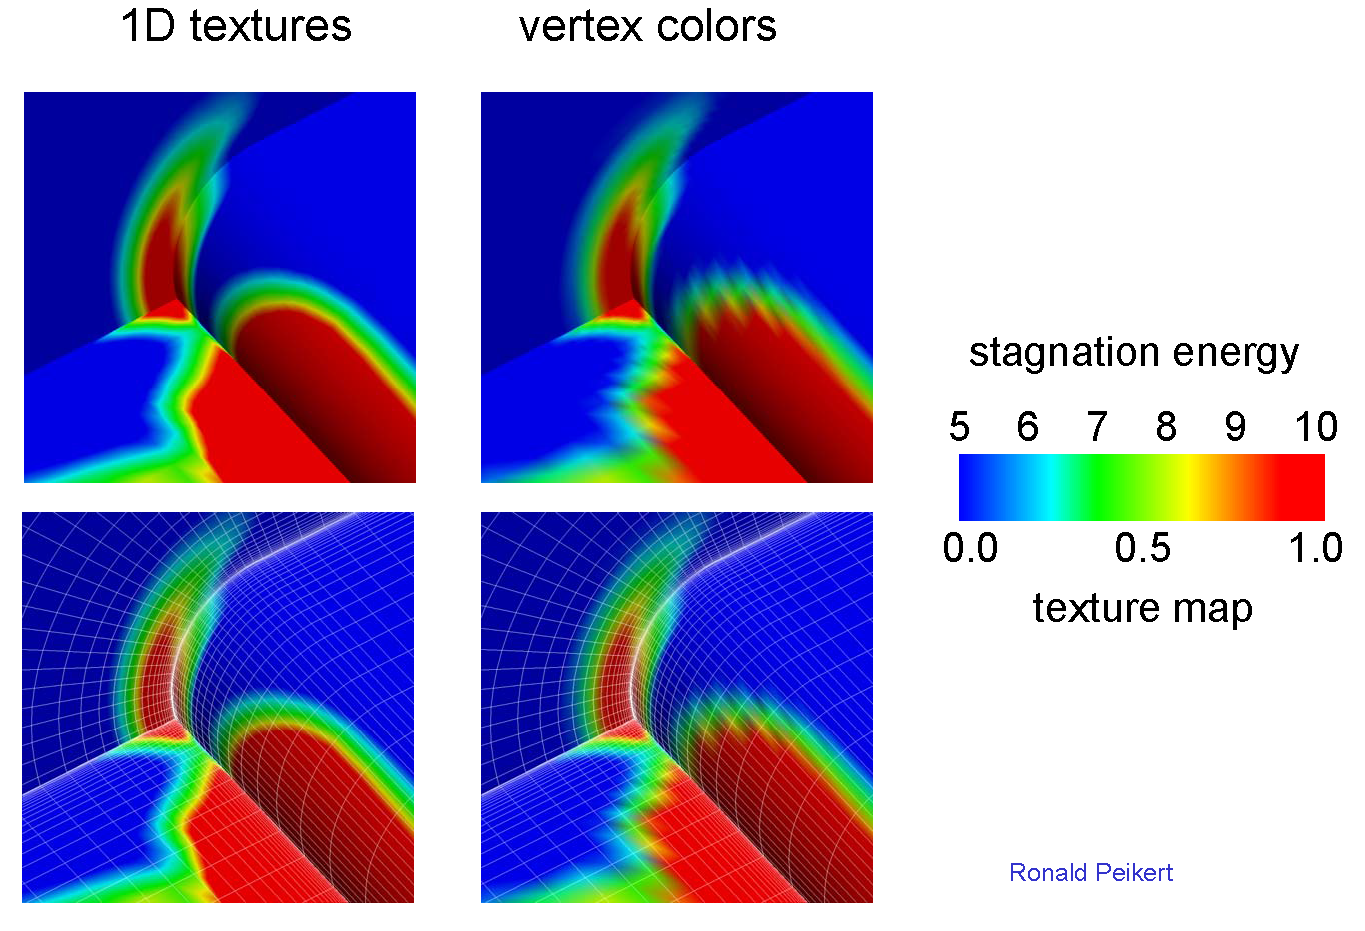
\includegraphics[width=0.9\textwidth]{img/01_texture_mapping}
\end{figure}

\begin{itemize}
    \item Problem of RGB colouring mode: The Interpolation is in the wrong colour space (RGB vs. colour table).
    \item  Problem of Colour Index mode: Lighting is not possible. 
\end{itemize}


